\documentclass[11pt]{article}
\usepackage[polish]{babel}
\usepackage[T1]{fontenc}
\usepackage[utf8]{inputenc}
\usepackage{graphicx}
\usepackage{enumitem}
\usepackage{fancyhdr}

\pagestyle{fancy}
\fancyhead[L]{Kacper Achramowicz\\
Projekt indywidualny AiSD}
\fancyhead[R]{09.XI.2020\\
V1.0}
\begin{document}

\begin{huge}
\begin{center}
\textbf{Specyfikacja funkcjonalna}
\end{center}
\end{huge}

 \renewcommand{\labelenumii}{\Roman{enumii}}
 \begin{enumerate}
 
 \item Opis ogólny
 
 \begin{enumerate}[label=\arabic{enumi}.\arabic*.]
 
 \item Nazwa programu\\
 Program nazywa się $VaccOpt$.
 \item Poruszany problem\\
 Program będzie optymalizował proces zakupu szczepionek przez hipotetyczne apteki.\\
 Każda z aptek będących pod opieką $GM$ ma podpisany kontrakt z każdym dystrybutorem szczepionek leczniczych.\\
 Program napisany przeze mnie (jako członka $ZA$) ma za zadanie korzystając z danych zawartych w pliku dostarczonym przez $GM$ ma znaleźć konfigurację, w której nastąpi minimalizacja kosztów sprzedaży szczepionek przy jednoczesnym zapewnieniu dostaw do wszystkich aptek.\\
 
 \item Użytkownik docelowy\\
 Przyjmując konwencję zadania użytkownikiem docelowym jest $GM$.\\
 Właściwym użytkownikiem docelowym naszego programu jest prowadzący zajęć laboratoryjnych.\\

 \end{enumerate}
 
 
 
\item Ogólna funkcjonalność

\begin{enumerate}[label=\arabic{enumi}.\arabic*.]
 \item  Korzystanie z programu\\
 Program wykonany jest w formie aplikacji działającej w terminalu. Do włączenia go wymagane jest posiadanie kompilatora Java.
\item  Uruchamianie programu\\
Aby włączyć program należy przejść w terminalu do katalogu zawierającego pilk wykonywalny \textbf{VaccOpt.jar} i włączyć go wpisując komendę \textsl{java -jar VaccOpt.jar "nazwaPliku"}, gdzie nazwaPliku to nazwa pliku z danymi. W przypadku wywołania bezargumentów program domyślnie przyjmuje korzyta z pliku \textsl{dane.txt}.
\item Możliwości programu\\
Program jest w stanie sprawdzić, czy przekazane mu $dane$ zgadzają się z ustalonymi dyrektywami, na ich podstawie zoptymalizować, czyli w tym wypadku zminimalizować koszty zaopatrzenia w pełni wszystkich aptek. Efektem końcowym działania programu jest wygenerowanie pliku $result.txt.$ 
\end{enumerate}
 
  \item Format danych i struktura plików
  
  \begin{enumerate}[label=\arabic{enumi}.\arabic*.]
  
 \item Słownik\\
$GM$ - grupa menadżerska\\
$ZA$ - zespół analityków\\
$Klucz$, $ID$ - element unikatowy dla każdej apteki oraz dystrybutora\\
$dane$ - w domyśle odpowiednio sformatowany plik dostarczony przez $GM$ lub jego zawartość\\
$GUI$ - graphical user interface, czyli interfejs graficzny widziany przez użytkownika\\
 
 \item Struktura katalogów\\
Cały kod tworzący program będzie znajdował się w w katalogu \textsl{src}, tam też będzie plik main.java. Wszystkie testy znajdować się będą w katalogu \textsl{test}. Przykładowe $dane$ będą znajdowały się w katalogu nadrzędnym dla\textsl{src} i \textsl{test}. Plik wyjściowy będzie generowany w tym samym folderze. 
\item Przechowywanie danych w programie \\
Sam program znajduje się w repozytorium Wydziału Elektrycznego Politechniki Warszawskiej.\\
W programie informacje pobrane z danych będą przechowywane postaci tablic $kluczy$, z którymi będą powiązane pozostałe informacje dotyczące aptek i dystybutorów. Jedna tablica zawierać będzie $klucze$ aptek, druga $klucze$ dystrybutorów. 
\item Dane wejściowe \\
Dane wejściowe znajdują się domyślnie w pliku dane.txt. Muszą zgadzać się one z przyjętym formatowaniem. Należy pamiętać, aby każda apteka i dystrybutor mieli $ID$. Dane w pliku muszą być oddzielone od siebie separatorem "|", a nazwy aptek i dystrybutorów nie mogą zawierać tego znaku. Każda z aptek musi mieć połączenie z każdym z dystrybutorów. Wszystke liczby zawarte w pliku muszą być liczbami dodatnimi, a zapotrzebowanie na szczepionki jak i ich dostępna ilość muszą być liczbami całkowitymi. Przykładowy plik wejściowy:\\

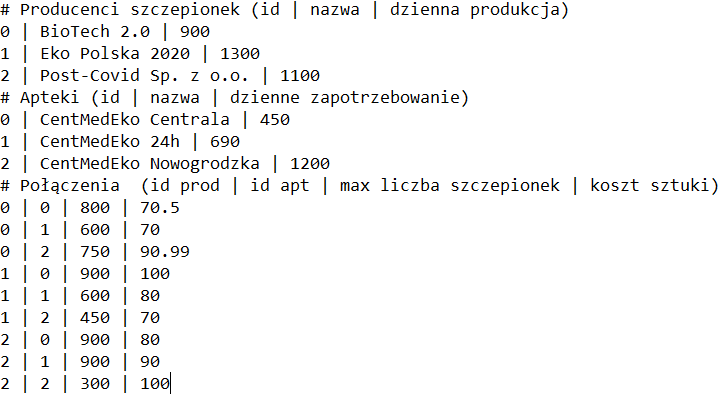
\includegraphics {in.png}

\item Dane wyjściowe\\
Dane wyjściowe znajdować się będą w pliku result.txt w poniższy sposób:

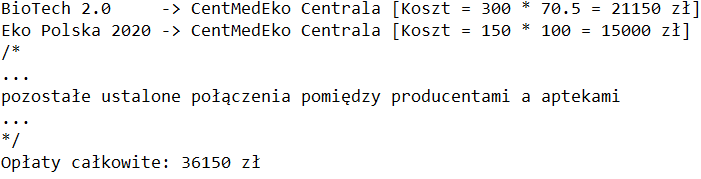
\includegraphics {out.png}



 \end{enumerate}
 

\item Scenariusz działania programu


\begin{enumerate}[label=\arabic{enumi}.\arabic*.]
\item Scenariusz ogólny
\begin{enumerate}[label*=\arabic*.]
\item Włączenie programu
\item Sprawdzenie, czy podany plik jest odpowiednio sformatowany
\item Wyliczenie namniejszego możliwego kosztu
\item Zapisanie danych do pliku wyjściowego
\item Koniec działania programu
\end{enumerate}
\item Scenariusz szczegółowy
\begin {enumerate}
\item Włączenie programu podając mu za argmunet własny plik z danymi, lub nie podając żadnego (wtedy pobierany jest plik domyślny)
\item Sprawdzenie przez program, czy plik jest odpowiednio sformatowany. Podanie informacji o błędzie jeżeli taki nie jest.
\item Zapisanie danych przez program w postaci tablic.
\item Sprawdzenie, w której konfiguracji dla każdej z aptek będzie najkorzystniej kupić szczepionki.
\item Optymalizacja tego procesu.
\item Sprawdzenie, czy można utworzyć plik wyjściowy i w przy pozytywnym rozpatrzeniu tego warunku utworzenie go. W przeciwnym wypadku komunikat błędu.
\item Zapisanie wyniku w poprawnym formacie do pliku result.txt
\item Zakończenie działania programu
\end{enumerate}




\end{enumerate}


 \item Testowanie\\
 \begin{enumerate}
 \item Ogólny przebieg testowania\\
 Do testów kodu użyty zostanie JUnit 4. Testy będą miały na celu sprawdzenie jak się zachowuje program w wypadku podania nieprawidłowego pliku przez $GM$ i czy zostanie zwrócona prawidłowa informacja o błędzie. Testy będą miały również sprawdzić, czy program zwraca prawidłowe dane i czy poprawnie tworzy nowe pliki wyjściowe.
 \end{enumerate}


\end{enumerate}



\end{document}